\documentclass[handout,nooutcomes,noauthor,hints]{ximera}

\graphicspath{  
{./}
{./whoAreYou/}
{./drawingWithTheTurtle/}
{./bisectionMethod/}
{./circles/}
{./anglesAndRightTriangles/}
{./lawOfSines/}
{./lawOfCosines/}
{./plotter/}
{./staircases/}
{./pitch/}
{./qualityControl/}
{./symmetry/}
{./nGonBlock/}
}


%% page layout
\usepackage[cm,headings]{fullpage}
\raggedright
\setlength\headheight{13.6pt}


%% fonts
\usepackage{euler}

\usepackage{FiraMono}
\renewcommand\familydefault{\ttdefault} 
\usepackage[defaultmathsizes]{mathastext}
\usepackage[htt]{hyphenat}

\usepackage[T1]{fontenc}
\usepackage[scaled=1]{FiraSans}

%\usepackage{wedn}
\usepackage{pbsi} %% Answer font


\usepackage{cancel} %% strike through in pitch/pitch.tex


%% \usepackage{ulem} %% 
%% \renewcommand{\ULthickness}{2pt}% changes underline thickness

\tikzset{>=stealth}

\usepackage{adjustbox}

\setcounter{titlenumber}{-1}

%% journal style
\makeatletter
\newcommand\journalstyle{%
  \def\activitystyle{activity-chapter}
  \def\maketitle{%
    \addtocounter{titlenumber}{1}%
                {\flushleft\small\sffamily\bfseries\@pretitle\par\vspace{-1.5em}}%
                {\flushleft\LARGE\sffamily\bfseries\thetitlenumber\hspace{1em}\@title \par }%
                {\vskip .6em\noindent\textit\theabstract\setcounter{question}{0}\setcounter{sectiontitlenumber}{0}}%
                    \par\vspace{2em}
                    \phantomsection\addcontentsline{toc}{section}{\thetitlenumber\hspace{1em}\textbf{\@title}}%
                     }}
\makeatother



%% thm like environments
\let\question\relax
\let\endquestion\relax

\newtheoremstyle{QuestionStyle}{\topsep}{\topsep}%%% space between body and thm
		{}                      %%% Thm body font
		{}                              %%% Indent amount (empty = no indent)
		{\bfseries}            %%% Thm head font
		{)}                              %%% Punctuation after thm head
		{ }                           %%% Space after thm head
		{\thmnumber{#2}\thmnote{ \bfseries(#3)}}%%% Thm head spec
\theoremstyle{QuestionStyle}
\newtheorem{question}{}



\let\freeResponse\relax
\let\endfreeResponse\relax

%% \newtheoremstyle{ResponseStyle}{\topsep}{\topsep}%%% space between body and thm
%% 		{\wedn\bfseries}                      %%% Thm body font
%% 		{}                              %%% Indent amount (empty = no indent)
%% 		{\wedn\bfseries}            %%% Thm head font
%% 		{}                              %%% Punctuation after thm head
%% 		{3ex}                           %%% Space after thm head
%% 		{\underline{\underline{\thmname{#1}}}}%%% Thm head spec
%% \theoremstyle{ResponseStyle}

\usepackage[tikz]{mdframed}
\mdfdefinestyle{ResponseStyle}{leftmargin=1cm,linecolor=black,roundcorner=5pt,
, font=\bsifamily,}%font=\wedn\bfseries\upshape,}


\ifhandout
\NewEnviron{freeResponse}{}
\else
%\newtheorem{freeResponse}{Response:}
\newenvironment{freeResponse}{\begin{mdframed}[style=ResponseStyle]}{\end{mdframed}}
\fi



%% attempting to automate outcomes.

%% \newwrite\outcomefile
%%   \immediate\openout\outcomefile=\jobname.oc
%% \renewcommand{\outcome}[1]{\edef\theoutcomes{\theoutcomes #1~}%
%% \immediate\write\outcomefile{\unexpanded{\outcome}{#1}}}

%% \newcommand{\outcomelist}{\begin{itemize}\theoutcomes\end{itemize}}

%% \NewEnviron{listOutcomes}{\small\sffamily
%% After answering the following questions, students should be able to:
%% \begin{itemize}
%% \BODY
%% \end{itemize}
%% }
\usepackage[tikz]{mdframed}
\mdfdefinestyle{OutcomeStyle}{leftmargin=2cm,rightmargin=2cm,linecolor=black,roundcorner=5pt,
, font=\small\sffamily,}%font=\wedn\bfseries\upshape,}
\newenvironment{listOutcomes}{\begin{mdframed}[style=OutcomeStyle]After answering the following questions, students should be able to:\begin{itemize}}{\end{itemize}\end{mdframed}}



%% my commands

\newcommand{\snap}{{\bfseries\itshape\textsf{Snap!}}}
\newcommand{\flavor}{\link[\snap]{https://snap.berkeley.edu/}}
\newcommand{\mooculus}{\textsf{\textbf{MOOC}\textnormal{\textsf{ULUS}}}}


\usepackage{tkz-euclide}
\tikzstyle geometryDiagrams=[rounded corners=.5pt,ultra thick,color=black]
\colorlet{penColor}{black} % Color of a curve in a plot



\ifhandout\newcommand{\mynewpage}{\newpage}\else\newcommand{\mynewpage}{}\fi

\title{Minifigs and superfigs}

\author{Claire Merriman}

\begin{document}
\begin{abstract}
  We extend scaling ideas from squares and cubes to arbitrary shapes,
  working with a real world example.
\end{abstract}
\maketitle

\begin{listOutcomes}
\item Apply the relation between linear scaling and area scaling,
\item Apply the relation between linear scaling and volume scaling,
\item Connect scaling of length, area, and volume to real-world attributes of objects,
\item Apply understanding of scaling to evaluate thought experiments.
\end{listOutcomes}

%% \begin{listObjectives}
%%  \item Explain the relationship between scaling lengths and scaling areas and volumes,
%% \item Learn and apply basic geometric formulas.
%% \end{listObjectives}

Here at the dimensions of a standard LEGO minifigure. Image and
additional measurements from
\url{https://www.flickr.com/photos/61628236@N05/8354305365/}
\begin{center}
 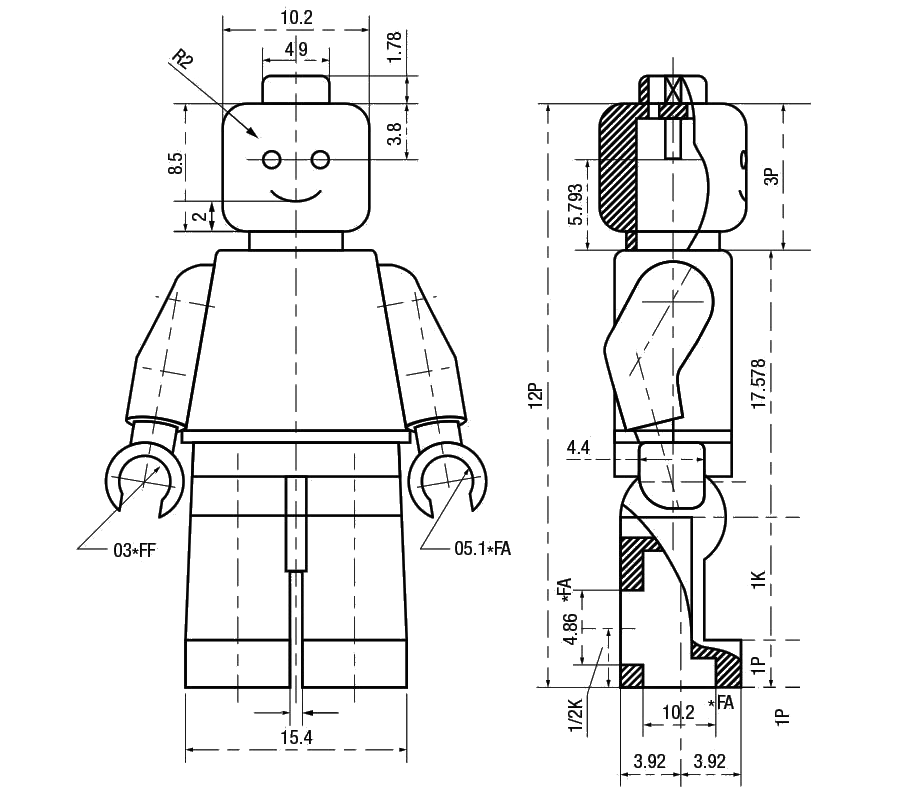
\includegraphics[height=.55\textheight]{lego-minifigure.png}
\end{center}

\mynewpage
\begin{question}
 This Instructables article explains how to make a ``giant'' LEGO man
 out of wood:
 \url{https://www.instructables.com/Giant-wooden-Lego-men/}
 
 He says that he uses a $1:6.25$ ratio for the scaling. 
 
\begin{enumerate}
 \item The original LEGO minifigure is $4$ centimeters tall. How tall is the
   wooden model?
 %% \item The head of the original LEGO minifigure is $10.2\ mm$ in
%%    diameter. What is the diameter of the head of the wooden model?
%%  \item The ``main'' part of the head (that is, without the stud to connect
%%    to other LEGO parts) the original LEGO minifigure is $8.5\ mm$
%%    tall. What is the height of the head of the wooden model?
%% \item The stud on top of the head of the original LEGO minifigure is
%%   $4.9 \ mm$ in diameter and $1.8 \ mm$ high. What are the dimensions
%%   of the stud on the wooden model?
 \item The body of the wooden model is $50$ millimeters thick. How
   thick is the original LEGO minifigure?
 \item What is the scale factor for the surface area of a LEGO
   minifigure compared to the surface area of the wooden model?
 \item What is the scale factor for the volume of a LEGO
   minifigure compared to the volume of the wooden model?
 
\end{enumerate}
%For all parts, round to the nearest tenth of a millimeter.
\end{question}
\mynewpage

\begin{question}
 Say you want to make a life-size wooden LEGO man that is $1.75$
 meters tall.
 
\begin{enumerate}
 \item What is the scale factor from the original LEGO minifigure?
   What about from the wooden model in the Instructables article?
 \item What is the scale factor for the surface area of a LEGO
   minifigure compared to the surface area of the life-size figure?
 \item What is the scale factor for the volume of a LEGO
   minifigure compared to the volume of the life-size figure?
\end{enumerate}
 \end{question}
\mynewpage

\begin{question}
  Let's think about some physical properties of these superfigures.
  \begin{enumerate}
 \item The wooden model in the Instructables article was finished with
   a spray coating of lacquer.  How much more lacquer would the life-size model need? Why?
 \item Assuming the same materials are used for both, how much more
   would the life-size wooden model weigh than the one in the
   Instructables article?  How do you know?
\end{enumerate}
\end{question}


%% \mynewpage
%% \begin{question}\textbf{(Optional)}

%% Artist Frank Ippolito made a Realistic LEGO Mini Figure Costume: \url{http://www.frankippolito.com/portfolio/creepy-lego-figure/}.  

%% %\begin{figure}[h]
%% %\begin{center}
%% % 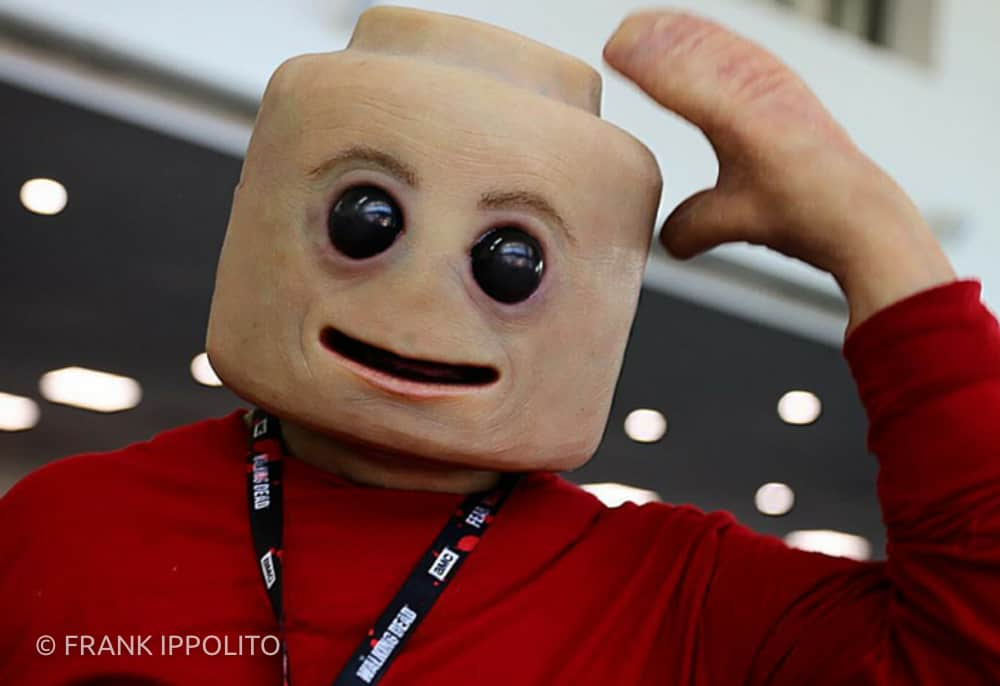
\includegraphics[width=.5\textwidth]{Frank_Ippolito_CreepyLegoFig.jpeg}
%% %\end{center}
%% %\end{figure}

%% These questions are about the mask part of the costume.  They go beyond the material covered in class, so are extra credit.
 
%% \begin{enumerate}
%%  \item Frank says that one way to determine the scale of the mask is to make sure that the eyes and mouth line up with his eyes and mouth\footnote{\url{https://www.youtube.com/watch?v=P2O7vyKnYfo}, starting around 5:08}. Let's assume that the eyes of the original LEGO minifigure are roughly $4.5 \ mm$ apart. 
 
%% According to this guide\footnote{\url{https://www.cvs.com/optical/article/how-to-measure-pupillary-distance}} for Measure Pupillary Distance (distance between pupils), the average pupillary distance for adults is between 54 and 74 millimeters. However, looking at the Creepy Fig mask, we can assume the center of the eyes are a bit wider apart than normal human eyes, maybe 90 mm. Assuming that everything else about the mask is to scale, what are the dimensions of the ``main" part of the head and the stud? Does this estimate seem realistic, based on the images of the mask?

%% \item What could be one explanation for why the numbers in part (a) are so different than the ones in Problem 2?

%% \item Say that instead of wearing the mask, Frank wanted to sculpt a body for Creepy Fig. Using the fact that the neck part of the original LEGO minifigure is $1.2\ mm$ tall, and assume that the neck of the mask is to scale, how tall would the body need to be for the model to be to scale?

%% \item If instead, Frank wanted to make a mask that was to scale for someone who is 6' tall, how far apart would the eyes be?
%%  \end{enumerate}
 
%\end{question}
\end{document}
